\section{Potential limits in shared memory programing models}

In this section two technical aspects that can potentially affect the overall performance of applications conforming to the shared memory programing model are evaluated. The first is related to the performance of the computer's memory sub-system, and the second relates to the cost of the barriers required by parallel program to ensure correct results.
%\medskip


\subsection*{Stream Benchmark}

For a long time we have witness how CPUs are being getting faster much more quickly than the computer's memory sub-system. Modern multi-core processors have become voracious consumers of data, and, as a consequence, more and more programs are being limited in performance by the memory bandwidth of the system, rather than by the computational performance of the CPU\cite{McCalpin2007}. It is, therefore, particularly important to be able to determine the memory bandwidth of the system at hand. 

\medskip


The STREAM benchmark\cite{McCalpin2007} is a suite of four (Copy, Scale, Add and Triad) simple tests that measures sustainable memory bandwidth (in MB/s) and the corresponding computation rate for simple vector kernels. In general, it is used to measure the evolution of the memory bandwidth of shared memory systems as more computing component are included in the test. Traditionally, the test has been implemented using OpenMP and the computing component are usually referred as threads.

\medskip

For MPI$_{sm}$ to become a viable alternative to OpenMP in the context of the shared memory programing model, it is fundamental that its sustainable memory bandwidth compares favorably to its OpenMP counterpart.

\medskip

The stream program that can be download from its web site \cite{McCalpin2007} is already annotated with directives (\textbf{\#pragma}) to make it a correct OpenMP program. This program was modified in order to develop an equivalent  MPI$_{sm}$ version. Both programs were run, using various compilers and MPI implementations. Some results, as well as lessons learned, follow.

\medskip

Figure \ref{fig:TriadTestBefore} presents results obtained on one system (\textbf{stout}) for the Triad test of the stream suite; results of the other tests (Copy, Scale and Add) are similar. The left plot, (\ref{fig:TriadBefore}) shows the actual bandwidth achieved while the right plot (\ref{fig:TriadRatioBefore}) show the MPI$_{sm}$ to OpenMP ratio obtained.
 
\medskip

\begin{figure} [h!]
    \centering
    \captionsetup{justification=centering, singlelinecheck=false}
    \begin{subfigure}{.6\textwidth}
      \hspace*{-1.5cm} 
      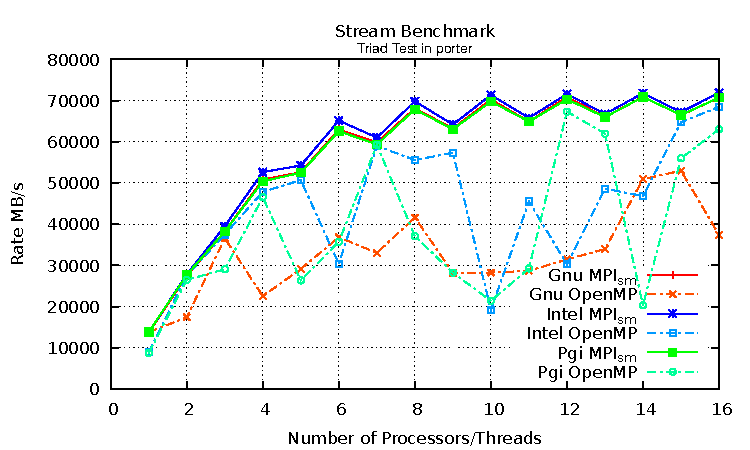
\includegraphics[width=0.95\linewidth]{Plots/streamBenchmark/porter-TriadBefore.pdf}
      \caption[]{Bandwidth per number of processes/threads.}
      \label{fig:TriadBefore}
    \end{subfigure}%
    \begin{subfigure}{.6\textwidth}
      \hspace*{-1.5cm} 
      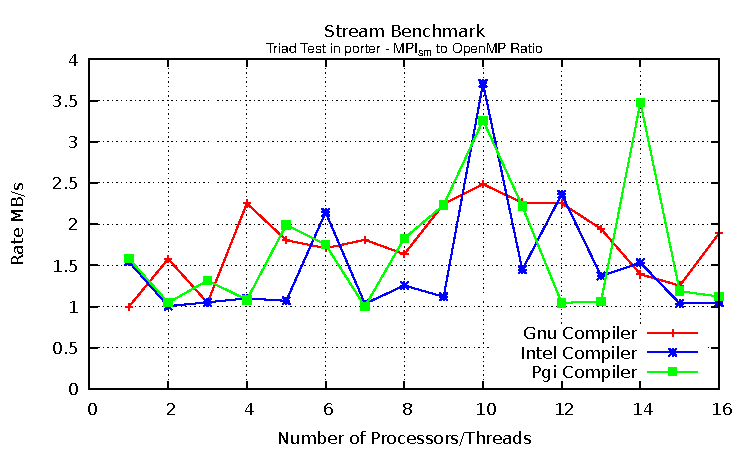
\includegraphics[width=0.95\linewidth]{Plots/streamBenchmark/porter-TriadRatioBefore.pdf}
      \caption{Ratio MPI$_{sm}$ to OpenMP.}
      \label{fig:TriadRatioBefore}
    \end{subfigure}
    \caption{Triad test. No binding policy for OpenMP}
\label{fig:TriadTestBefore}
\end{figure}


In Figure \ref{fig:TriadBefore} the segmented lines correspond to OpenMP while the continuous lines represent MPI$_{sm}$. Notice the extremely irregular behavior shown by all the OpenMP cases. Exploring the causes of such behavior lead to the first lesson in this section: \textbf{thread placement}. As mentioned in the Introduction, all the systems used in this study corresponds to systems having more than one socket. In this kind of systems, application having multiple threads could run into affinity problems.

\medskip

The lack of a \emph{by-default} thread affinity control policy of all the compilers used in the study results the erratic behavior shown in the Figure \ref{fig:TriadBefore}, because the threads are allow to be moved, by the OS, not only to a different core but also to a different socket. On the other hand, the more stable behavior that can be observed for the MPI$_{sm}$ case is due to the fact that the MPI implementations used \emph{do} have a \emph{by-default} binding policy for the processes running in the node.

\medskip

The ways to control thread affinity in OpenMP used to be compiler-dependent. However, OpenMP version 4.0 specification introduced a standardized mean to control thread affinity allowing, for the first time, an uniform way to have fine grain control over the affinity policy to compilers conforming to the standard. It introduced two new concepts: binding policy and place partition.

The binding policy determines if the threads will be bound and how they will be distributed, while the place partition is the set of places to which threads can be bound. One simple way of control the binding policy is by setting the \textbf{\texttt{OMP\_PROC\_BIND}} environment variable. Similarly, a way of control the place partition is by setting the \textbf{\texttt{OMP\_PLACES}} environment variable. 

\medskip

In our case, we found convenient to set 

\begin{itemize} 

\item \textbf{\texttt{OMP\_PROC\_BIND}}=spread 

\item \textbf{\texttt{OMP\_PLACES}}=sockets

\end{itemize}

meaning that the threads will be bound and distributed (or spread) among the sockets. More details about the values allowed for these enviromantal variables can be found in the current OpenMP API specification.

\medskip

Once a thread policy was set for the OpenMP cases, the stream tests were run again and the results are shown in Figure \ref{fig:TriadTest}. As before, the left plot, (\ref{fig:Triad}) shows the actual bandwidth achieved while the right plot (\ref{fig:TriadRatio}) show the MPI$_{sm}$ to OpenMP ratio obtained. 

\medskip
From the results shown in Figure \ref{fig:TriadTest} it can be seen that the sustainable memory bandwidth achievable by MPI$_{sm}$ is effectively at pair with its OpenMP counterpart.


\begin{figure} [h!]
    \centering
    \captionsetup{justification=centering, singlelinecheck=false}
    \begin{subfigure}{.6\textwidth}
      \hspace*{-1.5cm} 
      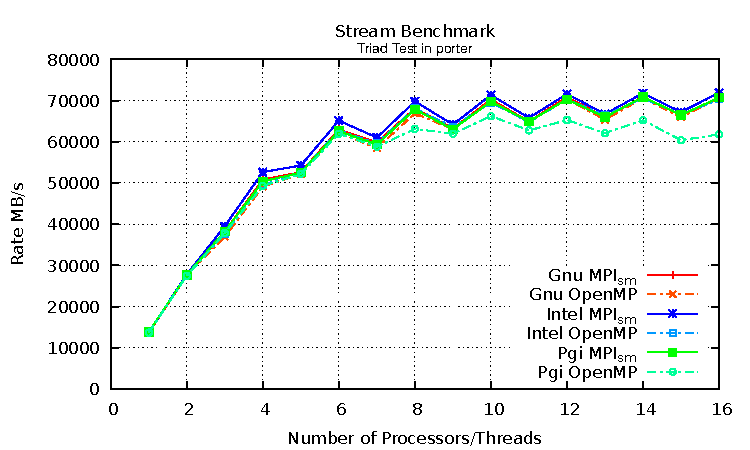
\includegraphics[width=0.95\linewidth]{Plots/streamBenchmark/porter-Triad.pdf}
      \caption[]{Bandwidth per number of processes/threads.}
      \label{fig:Triad}
    \end{subfigure}%
    \begin{subfigure}{.6\textwidth}
      \hspace*{-1.5cm} 
      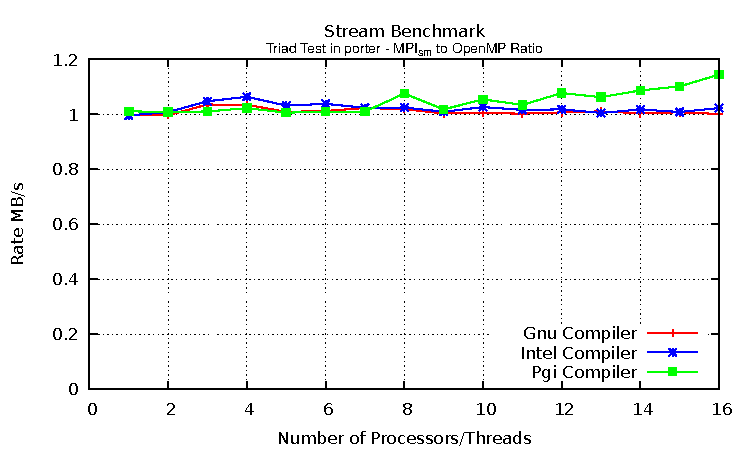
\includegraphics[width=0.95\linewidth]{Plots/streamBenchmark/porter-TriadRatio.pdf}
      \caption{Ratio MPI$_{sm}$ to OpenMP.}
      \label{fig:TriadRatio}
    \end{subfigure}
\caption{Triad test.}
\label{fig:TriadTest}
\end{figure}

\newpage

\subsection*{Barriers}
%causes a central processing unit (CPU) or compiler to enforce 

A memory barrier is a type of instruction that requires an ordering constraint on memory operations issued before and after it. They are necessary because most modern CPUs employ performance optimizations that can result in out-of-order execution. This reordering of memory operations (loads and stores) can produce incorrect results in parallel programs unless carefully controlled.

\medskip

The efficiency of the barrier implementation could potentially affect the overall performance of parallel applications conforming to the shared memory programing model. Therefore an effort was made to estimate, as accurate as possible, the time delay produced by the barrier itself, because a large difference in this delay between MPI$_{sm}$ and OpenMP could result crucial in choosing one or the other.

\medskip


Notice that what is being measured is not the time a particular thread/process wait in the barrier, which, in general, depends on the load unbalance; e.g. the time a thread/process is in the barrier waiting for its partners to arrive. However, the parameter being measured could be approximated by the minimum, among all the thread/process of the
time just described.




\medskip


\begin{figure} [h!]
\centering
\captionsetup{justification=centering, singlelinecheck=false}
    
\begin{lstlisting}[style=CStyle]
for (uint64_t n=0 ; n<max_iterations; ++n) {

    MPI_Barrier(sm_comm);
        
    clock_gettime(CLOCK_MONOTONIC, &start);
    MPI_Barrier(sm_comm);    
    clock_gettime(CLOCK_MONOTONIC, &end);
    
    diff = BILLION * (end.tv_sec - start.tv_sec) + end.tv_nsec - start.tv_nsec;
    MPI_Allreduce( MPI_IN_PLACE, &diff, 1, MPI_UNSIGNED_LONG, MPI_MIN,sm_comm);
    barrier_time+=diff;

}	// end for //
\end{lstlisting}    
\caption{Pseudo used to estimate MPI$_{sm}$ barrier time.}
\label{fig:PseudoCode3}
\end{figure}


\medskip


\begin{figure} [h!]
    \centering
    \captionsetup{justification=centering, singlelinecheck=false}
    \begin{subfigure}{.6\textwidth}
      \hspace*{-1.5cm} 
      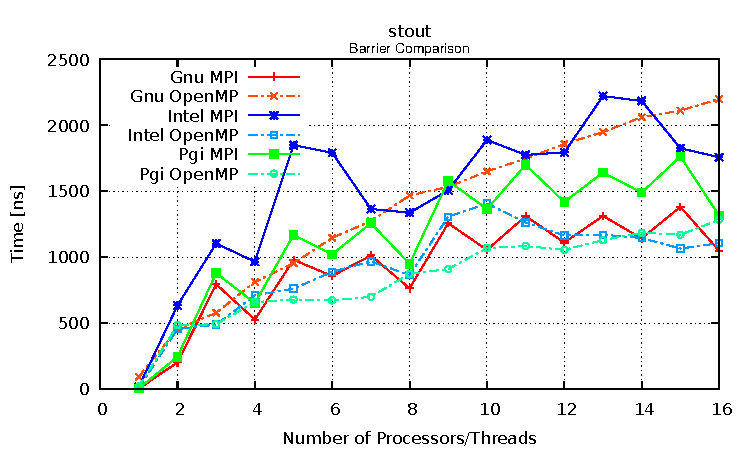
\includegraphics[width=0.95\linewidth]{Plots/barrier/stout.pdf}
      \caption[]{Estimated time.}
      \label{fig:Barrier}
    \end{subfigure}%
    \begin{subfigure}{.6\textwidth}
      \hspace*{-1.5cm} 
      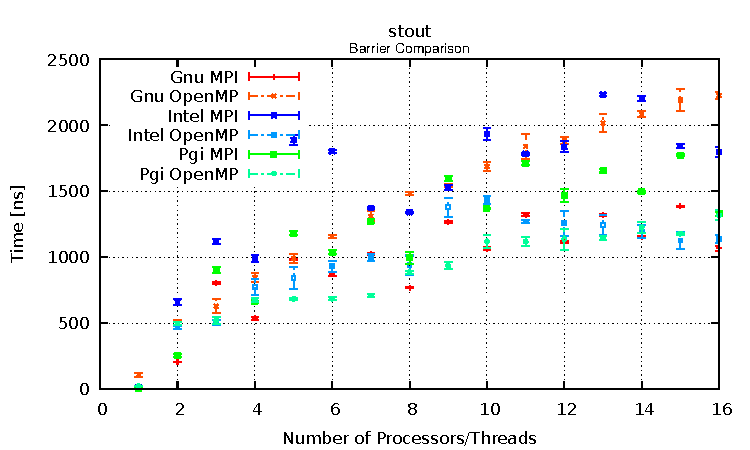
\includegraphics[width=0.95\linewidth]{Plots/barrier/stoutError.pdf}
      \caption{Errorbars to show variability of results.}
      \label{fig:BarrierErrorBars}
    \end{subfigure}
\caption{Barrier Results.}
\label{fig:BarrierAndErrorBars}
\end{figure}





\begin{comment}


Two identical versions of the stream benchmarks one using  and 
 were created and it 
 results are compared below for several systems. 
 
 
 However, the arrays 



 capabilities of the 

an MPI$_{sm}$ version of the program was developed and used to compare its performance to that obtained using its 



OpenMP versions of the STREAM benchmark program has been used to measure the evolution of the sustainable memory bandwidth of shared memory system as more threads are included in the test. 




What is STREAM?
The STREAM benchmark is a simple synthetic benchmark program that measures sustainable memory bandwidth (in MB/s) and the corresponding computation rate for simple vector kernels. 

Why should I care?

Computer cpus are getting faster much more quickly than computer memory systems. 

As this progresses, 

As an extreme example, several current high-end machines run simple arithmetic kernels for out-of-cache operands at 4-5 percent of their rated peak speeds --- that means that they are spending 95-96 percent of their time idle and waiting for cache misses to be satisfied.

The STREAM benchmark is specifically designed to work with datasets much larger than the available cache on any given system, so that the results are (presumably) more indicative of the performance of very large, vector style applications.

If you want more words, I have written a paper on STREAM: Sustainable Memory Bandwidth in Current High Performance Computers

A somewhat broader look on the issue, see my paper: Memory Bandwidth and Machine Balance in Current High Performance Computers. STREAM is also a useful component of models for scaling of homogeneous throughput workloads (like the SPEC CPU "rate" benchmarks). 

Examples of models based on STREAM measurements that do a pretty good job of estimating SPECfp rate2000 scaling are included in several presentations.

\end{comment}

